
\newpage
\section{Motifs}

In this chapter we analyze the strucarl. The term motif referes
to... . Studies of \textcite{Song2005} and \textcite{Perin2011} show
stuff. Pernice2011, Sporns , Zhao2011.

\newpage
\subsection*{Three-neuron patterns}

Here we investigate the occurrence of three-neuron patterns in
anisotropic networks. \textcite{Song2005} reported a characteristic,
highly non-random motif distribution of pyramidal cells in the rat's
visual cortex (layer 5), a result later confirmed by
\textcite{Perin2011} in their experiment in the rat's somatosensory
cortex (layer 5).

There are 13%
%------------------------------------
\footnote{%
  There are 16 simple directed with 3 nodes. Three of those graphs are
  unconnected \parencite[cf. ][%
  N. J. A. Sloane. The On-Line Encyclopedia of Integer Sequences,
  http://oeis.org. Sequence
  \href{http://oeis.org/A000273}{A000273}]{Davis1953}.%
} % 
%-------------------------------------
three-neuron motifs that represent non-isomorphic, connected simple
directed graphs. In reference to Song et al.'s result, the patterns
are labeled 4 to 16, \vspace{-0.2cm}
\begin{figure}[H]
  \centering
  \begin{overpic}[width=0.95\linewidth]{%
    plots/4839ce41_motifs_cropped.pdf}
  \put(100,0.2){.} 
  \end{overpic}
\end{figure}
\vspace{-0.8cm} Let $X$ be a random variable that maps three random
vertices $v_1 \neq v_2 \neq v_3$ in a graph $G$ to the $n \in
\{4,5,\dots,16\}$ labeling the isomorphism class of their spanned
subgraph in $G$ as above if the subgraph is connected, and let $X$ map
to $n=0$ otherwise. 

A first idea of how to compute the distribution of
$X$ is by inferring the probabilities of motif occurrence from the
two-neuron connection probabilities from
Section~\ref{sec:two_neuron}. In anisotropic networks we found that
the probabilities of occurrence are
\begin{align*} 
  p_u & = 0.791336     &&\text{for unconnected pairs,}     \\
  p_s & = 0.184151     &&\text{for single connections and} \\
  p_r & = 0.024513     &&\text{for reciprocal connections.}
\end{align*}
From these we may, for example, calculate the probability of
occurrence for motif 8, 
\[
  \mathbf{P}(X=8) = 6\, p_{u} p_{s} p_{r},
\]
where the factor 6 is determined by the number of different
\textit{labeled} graphs belonging to the isomorphism class. The
distribution of $X$ for the remaining motifs is given by
%
\vspace{-0.9cm}
\begin{figure}[H]
  \begin{minipage}[c]{0.32\textwidth}
    \begin{align*}
      % \mathbf{P}(X=1) &    =   p_u^3  \\
      % \mathbf{P}(X=2) &    =   6 p_u p_u p_s\\
      % \mathbf{P}(X=3) &    =   3 p_u p_u p_r\\
      \mathbf{P}(X=4) &    =   3 p_s^2 p_u\\
      \mathbf{P}(X=5) &    =   3 p_s^2 p_u\\
      \mathbf{P}(X=6) &    =   6 p_s^2 p_u\\
      \mathbf{P}(X=7) &    =   6 p_s p_u p_r
    \end{align*}
  \end{minipage}%
  \begin{minipage}[c]{0.32\textwidth}
    \begin{align*}
      \mathbf{P}(X=\,\,\,9) &    =   3 p_r^2 p_u\\
      \mathbf{P}(X=10) &   =   6 p_s^3   \\
      \mathbf{P}(X=11) &   =   2 p_s^3    \\
      \mathbf{P}(X=12) &   =   3 p_s^2 p_r
    \end{align*}
  \end{minipage}%
  \begin{minipage}[c]{0.32\textwidth}
    \begin{align*}
      \mathbf{P}(X=13) &   =   6 p_s^2 p_r\\
      \mathbf{P}(X=14) &   =   3 p_s^2 p_r\\
      \mathbf{P}(X=15) &   =   6 p_s p_r^2\\
      \mathbf{P}(X=16) &   =   p_r^3.
    \end{align*}
  \end{minipage}  
  \vspace{-0.9cm}
\end{figure}

Does this distribution accurately reflect the occurrences of
three-neuron motifs in anisotropic or even distance-dependent
networks? Here we take the distribution \marginpar{distribution from
  neuron-pairs as reference} determined from the two-neuron
probabilities as a reference to analyze occurrences of three-neuron
motifs in our sets of sample graphs. Counting the occurrences of
patterns in we find that there are significant over- and
underrepresentations in anisotropic as well as distance-dependent
networks, relative to our expectation
(\autoref{fig:3motif_single}). We find, for example, that in
anisotropic graphs pattern 12 occurs almost 5 times as often as we
would have expected from the two-neuron probabilities, whereas
the counts for pattern 11 only make up less than $30\%$ of the
occurrences expected.  

\begin{figure}[H]
  \centering
  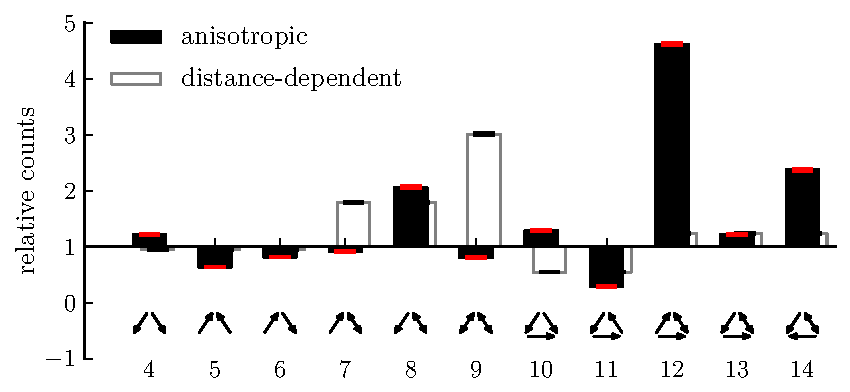
\includegraphics[width=0.95\linewidth]{%
    plots/4839ce41_aniso_dist.pdf}
  \captionsetup{skip=8pt}
  \caption{\textbf{Relative occurrence of three-neuron patterns}
    Extracting the counts of three-node motifs in anisotropic (filled
    bars) and distance-dependent networks (unfilled bars), the
    quotient of the obtained count with the number of occurrences
    expected from the two-neuron connection probabilities in the
    networks (cf. Section~\ref{sec:two_neuron}) shows the over- and
    underrepresentation of specific motifs in the network (red and
    black errorbars are SEM). In anisotropic networks pattern 12, for
    example, appears around five times more often than we would expect
    from the occurrence two-neuron connections. The relative counts
    for anisotropic networks resemble the findings of
    \textcite{Song2005} and differ significantly from the counts in
    distance-dependent networks, implying that anisotropy has a strong
    influence on the relative occurrence of three-neuron
    patterns. (\smtcite{4839ce41}) }
  \label{fig:3motif_single}
\end{figure}

This . \textcite{Perin2011} confirm the overrepresentation of motifs
4, 10, 12 and 14. In anisotropic networks we find increased counts of
motifs 4, 8, 10, 12, 13 and 14. However, comparison with motif counts in
distance-dependent networks shows that only the increased occurrence
of motif 4, 10, 12 and 14 


% Interestingly, full do not appear (mean = ) in tuned anisotropic,
% given evidence towards the incompleteness of the model.

% To fully we ex. The results from give good evidence, however we find
% that


\begin{figure}[H]
  \centering
  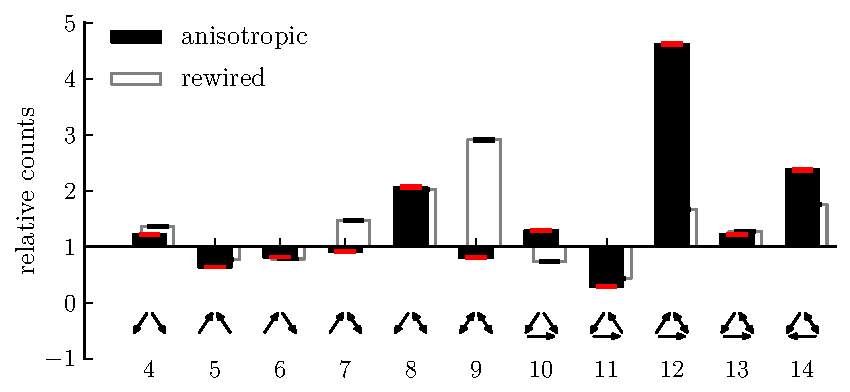
\includegraphics[width=0.95\linewidth]{%
    plots/4839ce41_aniso_rew.pdf}

  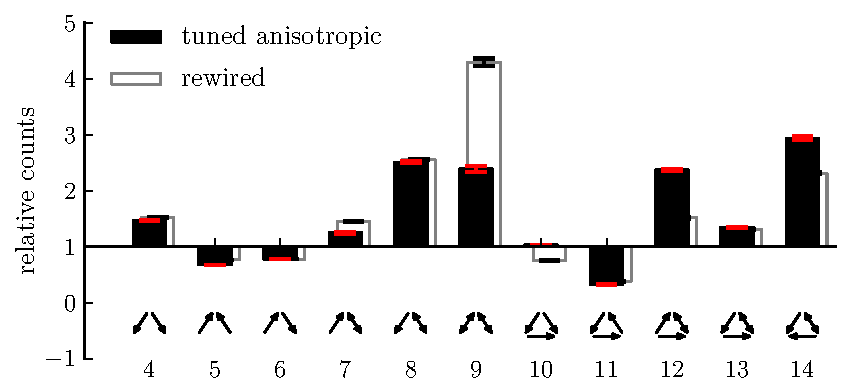
\includegraphics[width=0.95\linewidth]{%
    plots/4839ce41_tanfit_rew.pdf}

  \vspace{0.4cm}

  \makebox{%
    \hspace{1.208cm}%1.23
    \begin{overpic}[height=3.6cm]{%
        plots/4839ce41_motif15.pdf}
      \put(32.3,44.9){\small 15}
      \put(40,42.9){
\includegraphics[width=0.5cm]{img/misc/song_motif_15.pdf}}
    \end{overpic} 
    \hspace{0.19cm}
    \begin{overpic}[height=3.6cm]{%
        plots/4839ce41_motif16.pdf}
      \put(54,83){\small 16}
      \put(68,79){
\includegraphics[width=0.5cm]{img/misc/song_motif_16.pdf}}
    \end{overpic} 
  }%

  \captionsetup{skip=8pt}
  \caption{\textbf{Relative occurrence of three-neuron patterns}
    Extracting the counts of three-node motifs in anisotropic (filled
    bars) and distance-dependent networks (unfilled bars), the
    quotient of the obtained count with the number of occurrences
    expected from the two-neuron connection probabilities in the
    networks (cf. Section~\ref{sec:two_neuron}) shows the over- and
    underrepresentation of specific motifs in the network (red and
    black errorbars are SEM). In anisotropic networks pattern 12, for
    example, appears around five times more often than we would expect
    from the occurrence two-neuron connections. The relative counts
    for anisotropic networks resemble the findings of
    \textcite{Song2005} and differ significantly from the counts in
    distance-dependent networks, implying that anisotropy has a strong
    influence on the relative occurrence of three-neuron
    patterns. (\smtcite{4839ce41}) }
  \label{fig:3motif_full}
\end{figure}



Anisotropy in connectivity induces increased occurrence of motifs 10,
12, 14 and 15 in the network. It has strong influence the counts of
motif 16. While over- and underrepresentation observed in local
cortical circuits can be indirectly linked to anisotropy for some
motifs (4,11) it does not accurately reflect observed for other motifs
(8).



, however not
in motif 4. Additionally, anisotropy in connectivity causes for large
in motifs . Motif 9 is significantly underrepresented in anisotropic
networks, also reflecting the findings of Song et al. Overrep of 8 not
reported, here consistent through network types.





% \subsection*{Edge counts in neuron clusters}


% \begin{figure}[H]
%   \centering
%   \includegraphics[width=0.95\linewidth]{%
%     plots/7c826e10_test.pdf} 
%   \includegraphics[width=0.95\linewidth]{%
%     plots/Perin_test_6counts_compare.pdf} 
%   \captionsetup{skip=8pt}
%   \caption{\textbf{Relative foccurrence of three-neuron patterns}
%     Extracting the counts of three-node motifs in anisotropic (filled
%     bars) and distance-adependent networks (unfilled bars), the
%     quotient of the obtained count with the number of occurrences
%     expected from the two-neuron onnection probabilities in the
%     networks (rs =, ,, cfsdfg.) shows the over- and underrepresentation of
%     specific motifs in the network (red and black errorbars are
%     SEM). In anisotropic networks pattern number \enquote{12}, for
%     example, appears around five times more often than we would expect
%     from the occurrele the findings of
%     \textcite{Song2005} and differ significantly from the counts in
%     distance-dependent networks, implying that anisotropy has a strong
%     influence on the relative occurrence of three-neuron
%     patterns. (\smtcite{4839ce41}) }
%   \label{fig:distance_theory_compare}
% \end{figure}



% \begin{figure}[H]
%   \centering
%   \renewcommand{\tabcolsep}{0pt}
%   \setlength\extrarowheight{0pt}
%   \begin{tabular}{ll}
%     \begin{overpic}[width=0.5\textwidth]{%
%         /users/hoffmann/research/cn_k_test.pdf}
%       %\put(12,56){\small $\eta = 0$}
%     \end{overpic}
%     &
%     \begin{overpic}[width=0.5\textwidth]{%
%         /users/hoffmann/research/cn_k_test.pdf}
%       %\put(12,56){\small $\eta = 0.25$}
%     \end{overpic}
%     \\
%     \begin{overpic}[width=0.5\textwidth]{%
%         /users/hoffmann/research/cn_k_test.pdf}
%       %\put(12,56){\small $\eta = 0.5$}
%     \end{overpic}
%     &
%     \begin{overpic}[width=0.5\textwidth]{%
%         /users/hoffmann/research/cn_k_test.pdf}
%       % \put(12,56){\small $\eta = 0.75$}
%       %\put(4,-4){\small$0$}\put(78,-4){\small$200$}
%     \end{overpic}
%     \\
%     % \begin{overpic}[width=0.28\textwidth]{%
%     %     plots/77995b6b_in100.pdf}
%     %   \put(12,56){\small $\eta = 1$}
%     %   \put(4,-4){\small$0$}\put(78,-4){\small$200$}
%     % \end{overpic}
%     % & 
%     % \begin{overpic}[width=0.28\textwidth]{%
%     %     plots/77995b6b_indst.pdf}
%     %   \put(12,56){\small distance}
%     %   \put(4,-4){\small$0$}\put(78,-4){\small$200$}
%     % \end{overpic}
%     % \\
%   \end{tabular}
%   \caption{\textbf{In-degxree distrbution not affected by varying
%       degrees of anisotropy} 
%     (\smtcite{77995b6b}). }
%   \label{fig:in_degree_rewiring}
% \end{figure}



% \begin{figure}[htp]
%   \centering
 
%   \makebox{%
%     \hspace{1.23cm}
%     \begin{overpic}[height=3.6cm]{%
%         plots/4839ce41_motif15.pdf}
%       \put(32.3,44.9){\small 15}
%       \put(40,42.9){
\includegraphics[width=0.5cm]{img/misc/song_motif_15.pdf}}
%     \end{overpic} 
%     \hspace{0.19cm}
%     \begin{overpic}[height=3.6cm]{%
%         plots/4839ce41_motif16.pdf}
%       \put(54,83){\small 16}
%       \put(68,79){
\includegraphics[width=0.5cm]{img/misc/song_motif_16.pdf}}
%     \end{overpic} 
%   }%
%   \captionsetup{skip=7pt}
%   \caption{\textbf{Distance-independent overrepresentation of
%       reciprocal connections} Compaison of occurrences of one- and
%     bidirectionally connected neuron apairs in the tuned anisotropic
%     networks (gray) with profiles found by Perin et al.~(red), shows
%     that overrepresentation of bidirectional pairs is
%     distance-independent and not connected to anisotropy.  \textbf{A)}
%     Overall connection probability. (\smtcite{875505b0})}
%   \label{fig:perinadsf}
% \end{figure}


%%% Local Variables: 
%%% mode: latex
%%% TeX-master: "../dplths_document"
%%% End: 
